\documentclass[11pt,border=5pt]{standalone}
\usepackage{fontspec}
\setmainfont{cmunrm.otf}[BoldFont=cmunbx.otf,ItalicFont=cmunti.otf,BoldItalicFont=cmunbi.otf]
\usepackage{amsmath}
\usepackage{unicode-math}
\setmathfont{NewCMMath-Regular.otf}
\usepackage{tikz}
\usetikzlibrary{arrows.meta,patterns,angles,quotes}
\begin{document}
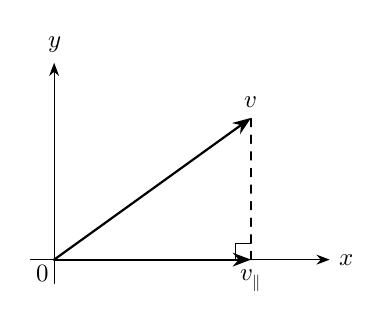
\begin{tikzpicture}[>=Stealth,font=\small,line cap=round,line join=round]
\draw[->,thin] (-0.3,0) -- (3.5,0) node[right] {$x$};
\draw[->,thin] (0,-0.3) -- (0,2.5) node[above] {$y$};
\node at (-0.14,-0.18) {$0$};
\draw[->,thick] (0,0) -- (2.5,1.8) node[above] {$v$};
\draw[->,thick] (0,0) -- (2.5,0) node[below] {$v_{\parallel}$};
\draw[dashed] (2.5,0) -- (2.5,1.8);
\draw(2.3,0)--(2.3,.2)--(2.5,.2);
\end{tikzpicture}
\end{document}
